% Created by tikzDevice version 0.12 on 2019-09-18 20:19:05
% !TEX encoding = UTF-8 Unicode
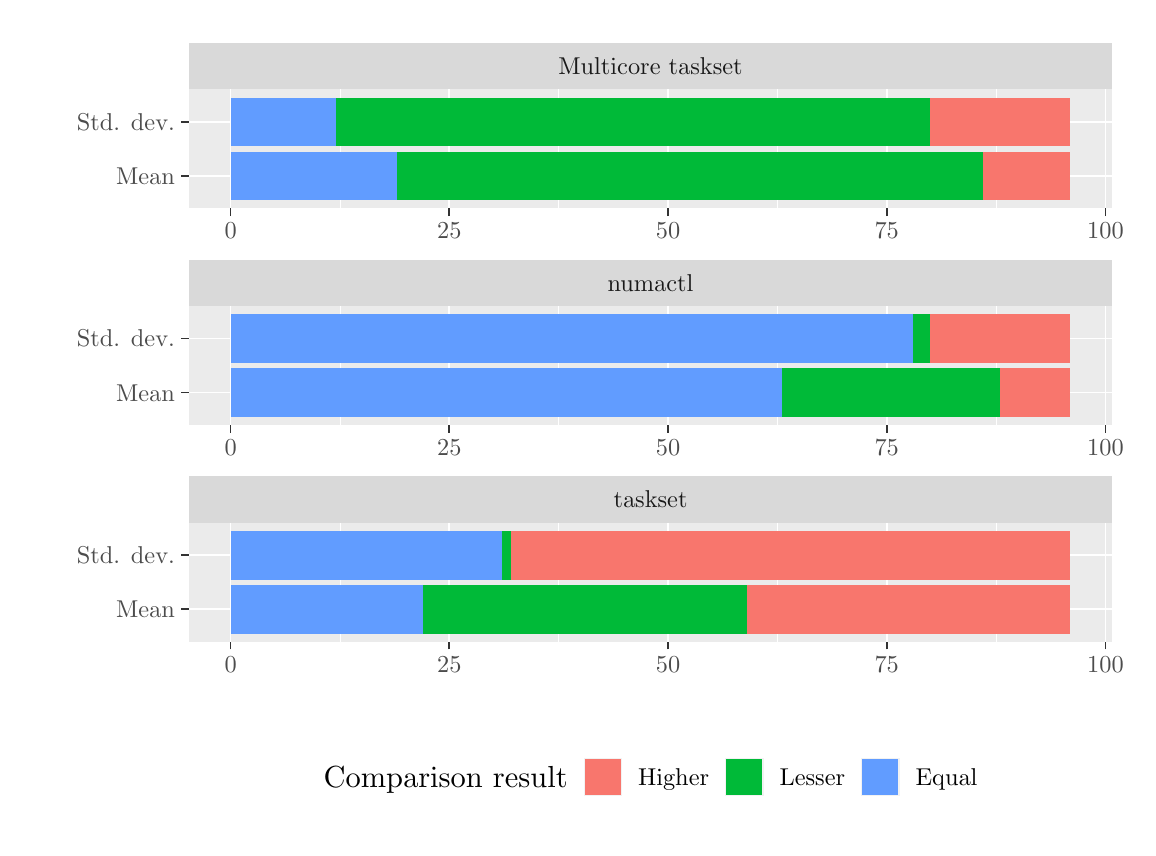
\begin{tikzpicture}[x=1pt,y=1pt]
\definecolor{fillColor}{RGB}{255,255,255}
\path[use as bounding box,fill=fillColor,fill opacity=0.00] (0,0) rectangle (397.48,289.08);
\begin{scope}
\path[clip] (  0.00,  0.00) rectangle (397.48,289.08);
\definecolor{drawColor}{RGB}{255,255,255}
\definecolor{fillColor}{RGB}{255,255,255}

\path[draw=drawColor,line width= 0.6pt,line join=round,line cap=round,fill=fillColor] (  0.00,  0.00) rectangle (397.48,289.08);
\end{scope}
\begin{scope}
\path[clip] ( 58.16,223.75) rectangle (391.98,266.78);
\definecolor{fillColor}{gray}{0.92}

\path[fill=fillColor] ( 58.16,223.75) rectangle (391.98,266.78);
\definecolor{drawColor}{RGB}{255,255,255}

\path[draw=drawColor,line width= 0.3pt,line join=round] (112.85,223.75) --
	(112.85,266.78);

\path[draw=drawColor,line width= 0.3pt,line join=round] (191.88,223.75) --
	(191.88,266.78);

\path[draw=drawColor,line width= 0.3pt,line join=round] (270.91,223.75) --
	(270.91,266.78);

\path[draw=drawColor,line width= 0.3pt,line join=round] (349.94,223.75) --
	(349.94,266.78);

\path[draw=drawColor,line width= 0.6pt,line join=round] ( 58.16,235.48) --
	(391.98,235.48);

\path[draw=drawColor,line width= 0.6pt,line join=round] ( 58.16,255.04) --
	(391.98,255.04);

\path[draw=drawColor,line width= 0.6pt,line join=round] ( 73.33,223.75) --
	( 73.33,266.78);

\path[draw=drawColor,line width= 0.6pt,line join=round] (152.36,223.75) --
	(152.36,266.78);

\path[draw=drawColor,line width= 0.6pt,line join=round] (231.39,223.75) --
	(231.39,266.78);

\path[draw=drawColor,line width= 0.6pt,line join=round] (310.42,223.75) --
	(310.42,266.78);

\path[draw=drawColor,line width= 0.6pt,line join=round] (389.46,223.75) --
	(389.46,266.78);
\definecolor{fillColor}{RGB}{97,156,255}

\path[fill=fillColor] ( 73.33,226.68) rectangle (133.39,244.28);
\definecolor{fillColor}{RGB}{0,186,56}

\path[fill=fillColor] (133.39,226.68) rectangle (345.20,244.28);
\definecolor{fillColor}{RGB}{248,118,109}

\path[fill=fillColor] (345.20,226.68) rectangle (376.81,244.28);
\definecolor{fillColor}{RGB}{97,156,255}

\path[fill=fillColor] ( 73.33,246.24) rectangle (111.27,263.84);
\definecolor{fillColor}{RGB}{0,186,56}

\path[fill=fillColor] (111.27,246.24) rectangle (326.23,263.84);
\definecolor{fillColor}{RGB}{248,118,109}

\path[fill=fillColor] (326.23,246.24) rectangle (376.81,263.84);
\end{scope}
\begin{scope}
\path[clip] ( 58.16,145.46) rectangle (391.98,188.49);
\definecolor{fillColor}{gray}{0.92}

\path[fill=fillColor] ( 58.16,145.46) rectangle (391.98,188.49);
\definecolor{drawColor}{RGB}{255,255,255}

\path[draw=drawColor,line width= 0.3pt,line join=round] (112.85,145.46) --
	(112.85,188.49);

\path[draw=drawColor,line width= 0.3pt,line join=round] (191.88,145.46) --
	(191.88,188.49);

\path[draw=drawColor,line width= 0.3pt,line join=round] (270.91,145.46) --
	(270.91,188.49);

\path[draw=drawColor,line width= 0.3pt,line join=round] (349.94,145.46) --
	(349.94,188.49);

\path[draw=drawColor,line width= 0.6pt,line join=round] ( 58.16,157.20) --
	(391.98,157.20);

\path[draw=drawColor,line width= 0.6pt,line join=round] ( 58.16,176.76) --
	(391.98,176.76);

\path[draw=drawColor,line width= 0.6pt,line join=round] ( 73.33,145.46) --
	( 73.33,188.49);

\path[draw=drawColor,line width= 0.6pt,line join=round] (152.36,145.46) --
	(152.36,188.49);

\path[draw=drawColor,line width= 0.6pt,line join=round] (231.39,145.46) --
	(231.39,188.49);

\path[draw=drawColor,line width= 0.6pt,line join=round] (310.42,145.46) --
	(310.42,188.49);

\path[draw=drawColor,line width= 0.6pt,line join=round] (389.46,145.46) --
	(389.46,188.49);
\definecolor{fillColor}{RGB}{97,156,255}

\path[fill=fillColor] ( 73.33,148.40) rectangle (272.49,166.00);
\definecolor{fillColor}{RGB}{0,186,56}

\path[fill=fillColor] (272.49,148.40) rectangle (351.52,166.00);
\definecolor{fillColor}{RGB}{248,118,109}

\path[fill=fillColor] (351.52,148.40) rectangle (376.81,166.00);
\definecolor{fillColor}{RGB}{97,156,255}

\path[fill=fillColor] ( 73.33,167.95) rectangle (319.91,185.56);
\definecolor{fillColor}{RGB}{0,186,56}

\path[fill=fillColor] (319.91,167.95) rectangle (326.23,185.56);
\definecolor{fillColor}{RGB}{248,118,109}

\path[fill=fillColor] (326.23,167.95) rectangle (376.81,185.56);
\end{scope}
\begin{scope}
\path[clip] ( 58.16, 67.18) rectangle (391.98,110.20);
\definecolor{fillColor}{gray}{0.92}

\path[fill=fillColor] ( 58.16, 67.18) rectangle (391.98,110.20);
\definecolor{drawColor}{RGB}{255,255,255}

\path[draw=drawColor,line width= 0.3pt,line join=round] (112.85, 67.18) --
	(112.85,110.20);

\path[draw=drawColor,line width= 0.3pt,line join=round] (191.88, 67.18) --
	(191.88,110.20);

\path[draw=drawColor,line width= 0.3pt,line join=round] (270.91, 67.18) --
	(270.91,110.20);

\path[draw=drawColor,line width= 0.3pt,line join=round] (349.94, 67.18) --
	(349.94,110.20);

\path[draw=drawColor,line width= 0.6pt,line join=round] ( 58.16, 78.91) --
	(391.98, 78.91);

\path[draw=drawColor,line width= 0.6pt,line join=round] ( 58.16, 98.47) --
	(391.98, 98.47);

\path[draw=drawColor,line width= 0.6pt,line join=round] ( 73.33, 67.18) --
	( 73.33,110.20);

\path[draw=drawColor,line width= 0.6pt,line join=round] (152.36, 67.18) --
	(152.36,110.20);

\path[draw=drawColor,line width= 0.6pt,line join=round] (231.39, 67.18) --
	(231.39,110.20);

\path[draw=drawColor,line width= 0.6pt,line join=round] (310.42, 67.18) --
	(310.42,110.20);

\path[draw=drawColor,line width= 0.6pt,line join=round] (389.46, 67.18) --
	(389.46,110.20);
\definecolor{fillColor}{RGB}{97,156,255}

\path[fill=fillColor] ( 73.33, 70.11) rectangle (142.88, 87.71);
\definecolor{fillColor}{RGB}{0,186,56}

\path[fill=fillColor] (142.88, 70.11) rectangle (259.84, 87.71);
\definecolor{fillColor}{RGB}{248,118,109}

\path[fill=fillColor] (259.84, 70.11) rectangle (376.81, 87.71);
\definecolor{fillColor}{RGB}{97,156,255}

\path[fill=fillColor] ( 73.33, 89.67) rectangle (171.33,107.27);
\definecolor{fillColor}{RGB}{0,186,56}

\path[fill=fillColor] (171.33, 89.67) rectangle (174.49,107.27);
\definecolor{fillColor}{RGB}{248,118,109}

\path[fill=fillColor] (174.49, 89.67) rectangle (376.81,107.27);
\end{scope}
\begin{scope}
\path[clip] ( 58.16,110.20) rectangle (391.98,127.01);
\definecolor{fillColor}{gray}{0.85}

\path[fill=fillColor] ( 58.16,110.20) rectangle (391.98,127.01);
\definecolor{drawColor}{gray}{0.10}

\node[text=drawColor,anchor=base,inner sep=0pt, outer sep=0pt, scale=  0.88] at (225.07,115.58) {taskset};
\end{scope}
\begin{scope}
\path[clip] ( 58.16,188.49) rectangle (391.98,205.29);
\definecolor{fillColor}{gray}{0.85}

\path[fill=fillColor] ( 58.16,188.49) rectangle (391.98,205.29);
\definecolor{drawColor}{gray}{0.10}

\node[text=drawColor,anchor=base,inner sep=0pt, outer sep=0pt, scale=  0.88] at (225.07,193.86) {numactl};
\end{scope}
\begin{scope}
\path[clip] ( 58.16,266.78) rectangle (391.98,283.58);
\definecolor{fillColor}{gray}{0.85}

\path[fill=fillColor] ( 58.16,266.78) rectangle (391.98,283.58);
\definecolor{drawColor}{gray}{0.10}

\node[text=drawColor,anchor=base,inner sep=0pt, outer sep=0pt, scale=  0.88] at (225.07,272.15) {Multicore taskset};
\end{scope}
\begin{scope}
\path[clip] (  0.00,  0.00) rectangle (397.48,289.08);
\definecolor{drawColor}{gray}{0.20}

\path[draw=drawColor,line width= 0.6pt,line join=round] ( 73.33, 64.43) --
	( 73.33, 67.18);

\path[draw=drawColor,line width= 0.6pt,line join=round] (152.36, 64.43) --
	(152.36, 67.18);

\path[draw=drawColor,line width= 0.6pt,line join=round] (231.39, 64.43) --
	(231.39, 67.18);

\path[draw=drawColor,line width= 0.6pt,line join=round] (310.42, 64.43) --
	(310.42, 67.18);

\path[draw=drawColor,line width= 0.6pt,line join=round] (389.46, 64.43) --
	(389.46, 67.18);
\end{scope}
\begin{scope}
\path[clip] (  0.00,  0.00) rectangle (397.48,289.08);
\definecolor{drawColor}{gray}{0.30}

\node[text=drawColor,anchor=base,inner sep=0pt, outer sep=0pt, scale=  0.88] at ( 73.33, 56.17) {0};

\node[text=drawColor,anchor=base,inner sep=0pt, outer sep=0pt, scale=  0.88] at (152.36, 56.17) {25};

\node[text=drawColor,anchor=base,inner sep=0pt, outer sep=0pt, scale=  0.88] at (231.39, 56.17) {50};

\node[text=drawColor,anchor=base,inner sep=0pt, outer sep=0pt, scale=  0.88] at (310.42, 56.17) {75};

\node[text=drawColor,anchor=base,inner sep=0pt, outer sep=0pt, scale=  0.88] at (389.46, 56.17) {100};
\end{scope}
\begin{scope}
\path[clip] (  0.00,  0.00) rectangle (397.48,289.08);
\definecolor{drawColor}{gray}{0.20}

\path[draw=drawColor,line width= 0.6pt,line join=round] ( 73.33,142.71) --
	( 73.33,145.46);

\path[draw=drawColor,line width= 0.6pt,line join=round] (152.36,142.71) --
	(152.36,145.46);

\path[draw=drawColor,line width= 0.6pt,line join=round] (231.39,142.71) --
	(231.39,145.46);

\path[draw=drawColor,line width= 0.6pt,line join=round] (310.42,142.71) --
	(310.42,145.46);

\path[draw=drawColor,line width= 0.6pt,line join=round] (389.46,142.71) --
	(389.46,145.46);
\end{scope}
\begin{scope}
\path[clip] (  0.00,  0.00) rectangle (397.48,289.08);
\definecolor{drawColor}{gray}{0.30}

\node[text=drawColor,anchor=base,inner sep=0pt, outer sep=0pt, scale=  0.88] at ( 73.33,134.45) {0};

\node[text=drawColor,anchor=base,inner sep=0pt, outer sep=0pt, scale=  0.88] at (152.36,134.45) {25};

\node[text=drawColor,anchor=base,inner sep=0pt, outer sep=0pt, scale=  0.88] at (231.39,134.45) {50};

\node[text=drawColor,anchor=base,inner sep=0pt, outer sep=0pt, scale=  0.88] at (310.42,134.45) {75};

\node[text=drawColor,anchor=base,inner sep=0pt, outer sep=0pt, scale=  0.88] at (389.46,134.45) {100};
\end{scope}
\begin{scope}
\path[clip] (  0.00,  0.00) rectangle (397.48,289.08);
\definecolor{drawColor}{gray}{0.20}

\path[draw=drawColor,line width= 0.6pt,line join=round] ( 73.33,221.00) --
	( 73.33,223.75);

\path[draw=drawColor,line width= 0.6pt,line join=round] (152.36,221.00) --
	(152.36,223.75);

\path[draw=drawColor,line width= 0.6pt,line join=round] (231.39,221.00) --
	(231.39,223.75);

\path[draw=drawColor,line width= 0.6pt,line join=round] (310.42,221.00) --
	(310.42,223.75);

\path[draw=drawColor,line width= 0.6pt,line join=round] (389.46,221.00) --
	(389.46,223.75);
\end{scope}
\begin{scope}
\path[clip] (  0.00,  0.00) rectangle (397.48,289.08);
\definecolor{drawColor}{gray}{0.30}

\node[text=drawColor,anchor=base,inner sep=0pt, outer sep=0pt, scale=  0.88] at ( 73.33,212.74) {0};

\node[text=drawColor,anchor=base,inner sep=0pt, outer sep=0pt, scale=  0.88] at (152.36,212.74) {25};

\node[text=drawColor,anchor=base,inner sep=0pt, outer sep=0pt, scale=  0.88] at (231.39,212.74) {50};

\node[text=drawColor,anchor=base,inner sep=0pt, outer sep=0pt, scale=  0.88] at (310.42,212.74) {75};

\node[text=drawColor,anchor=base,inner sep=0pt, outer sep=0pt, scale=  0.88] at (389.46,212.74) {100};
\end{scope}
\begin{scope}
\path[clip] (  0.00,  0.00) rectangle (397.48,289.08);
\definecolor{drawColor}{gray}{0.30}

\node[text=drawColor,anchor=base east,inner sep=0pt, outer sep=0pt, scale=  0.88] at ( 53.21,232.45) {Mean};

\node[text=drawColor,anchor=base east,inner sep=0pt, outer sep=0pt, scale=  0.88] at ( 53.21,252.01) {Std. dev.};
\end{scope}
\begin{scope}
\path[clip] (  0.00,  0.00) rectangle (397.48,289.08);
\definecolor{drawColor}{gray}{0.20}

\path[draw=drawColor,line width= 0.6pt,line join=round] ( 55.41,235.48) --
	( 58.16,235.48);

\path[draw=drawColor,line width= 0.6pt,line join=round] ( 55.41,255.04) --
	( 58.16,255.04);
\end{scope}
\begin{scope}
\path[clip] (  0.00,  0.00) rectangle (397.48,289.08);
\definecolor{drawColor}{gray}{0.30}

\node[text=drawColor,anchor=base east,inner sep=0pt, outer sep=0pt, scale=  0.88] at ( 53.21,154.17) {Mean};

\node[text=drawColor,anchor=base east,inner sep=0pt, outer sep=0pt, scale=  0.88] at ( 53.21,173.73) {Std. dev.};
\end{scope}
\begin{scope}
\path[clip] (  0.00,  0.00) rectangle (397.48,289.08);
\definecolor{drawColor}{gray}{0.20}

\path[draw=drawColor,line width= 0.6pt,line join=round] ( 55.41,157.20) --
	( 58.16,157.20);

\path[draw=drawColor,line width= 0.6pt,line join=round] ( 55.41,176.76) --
	( 58.16,176.76);
\end{scope}
\begin{scope}
\path[clip] (  0.00,  0.00) rectangle (397.48,289.08);
\definecolor{drawColor}{gray}{0.30}

\node[text=drawColor,anchor=base east,inner sep=0pt, outer sep=0pt, scale=  0.88] at ( 53.21, 75.88) {Mean};

\node[text=drawColor,anchor=base east,inner sep=0pt, outer sep=0pt, scale=  0.88] at ( 53.21, 95.44) {Std. dev.};
\end{scope}
\begin{scope}
\path[clip] (  0.00,  0.00) rectangle (397.48,289.08);
\definecolor{drawColor}{gray}{0.20}

\path[draw=drawColor,line width= 0.6pt,line join=round] ( 55.41, 78.91) --
	( 58.16, 78.91);

\path[draw=drawColor,line width= 0.6pt,line join=round] ( 55.41, 98.47) --
	( 58.16, 98.47);
\end{scope}
\begin{scope}
\path[clip] (  0.00,  0.00) rectangle (397.48,289.08);
\definecolor{fillColor}{RGB}{255,255,255}

\path[fill=fillColor] (101.43,  5.50) rectangle (348.71, 30.95);
\end{scope}
\begin{scope}
\path[clip] (  0.00,  0.00) rectangle (397.48,289.08);
\definecolor{drawColor}{RGB}{0,0,0}

\node[text=drawColor,anchor=base west,inner sep=0pt, outer sep=0pt, scale=  1.10] at (106.93, 14.44) {Comparison result};
\end{scope}
\begin{scope}
\path[clip] (  0.00,  0.00) rectangle (397.48,289.08);
\definecolor{drawColor}{RGB}{255,255,255}
\definecolor{fillColor}{gray}{0.95}

\path[draw=drawColor,line width= 0.6pt,line join=round,line cap=round,fill=fillColor] (200.59, 11.00) rectangle (215.05, 25.45);
\end{scope}
\begin{scope}
\path[clip] (  0.00,  0.00) rectangle (397.48,289.08);
\definecolor{fillColor}{RGB}{248,118,109}

\path[fill=fillColor] (201.31, 11.71) rectangle (214.34, 24.74);
\end{scope}
\begin{scope}
\path[clip] (  0.00,  0.00) rectangle (397.48,289.08);
\definecolor{drawColor}{RGB}{255,255,255}
\definecolor{fillColor}{gray}{0.95}

\path[draw=drawColor,line width= 0.6pt,line join=round,line cap=round,fill=fillColor] (251.73, 11.00) rectangle (266.19, 25.45);
\end{scope}
\begin{scope}
\path[clip] (  0.00,  0.00) rectangle (397.48,289.08);
\definecolor{fillColor}{RGB}{0,186,56}

\path[fill=fillColor] (252.45, 11.71) rectangle (265.48, 24.74);
\end{scope}
\begin{scope}
\path[clip] (  0.00,  0.00) rectangle (397.48,289.08);
\definecolor{drawColor}{RGB}{255,255,255}
\definecolor{fillColor}{gray}{0.95}

\path[draw=drawColor,line width= 0.6pt,line join=round,line cap=round,fill=fillColor] (300.89, 11.00) rectangle (315.35, 25.45);
\end{scope}
\begin{scope}
\path[clip] (  0.00,  0.00) rectangle (397.48,289.08);
\definecolor{fillColor}{RGB}{97,156,255}

\path[fill=fillColor] (301.60, 11.71) rectangle (314.64, 24.74);
\end{scope}
\begin{scope}
\path[clip] (  0.00,  0.00) rectangle (397.48,289.08);
\definecolor{drawColor}{RGB}{0,0,0}

\node[text=drawColor,anchor=base west,inner sep=0pt, outer sep=0pt, scale=  0.88] at (220.55, 15.20) {Higher};
\end{scope}
\begin{scope}
\path[clip] (  0.00,  0.00) rectangle (397.48,289.08);
\definecolor{drawColor}{RGB}{0,0,0}

\node[text=drawColor,anchor=base west,inner sep=0pt, outer sep=0pt, scale=  0.88] at (271.69, 15.20) {Lesser};
\end{scope}
\begin{scope}
\path[clip] (  0.00,  0.00) rectangle (397.48,289.08);
\definecolor{drawColor}{RGB}{0,0,0}

\node[text=drawColor,anchor=base west,inner sep=0pt, outer sep=0pt, scale=  0.88] at (320.85, 15.20) {Equal};
\end{scope}
\end{tikzpicture}
